\chapter*{Introduction}
\addcontentsline{toc}{chapter}{Introduction}

%Charming decore. Delicious food. Friendly staff. We'll certainly become repeat customers.", "useful": 2


With growing popularity of storing and sharing more data on the internet, the biggest challenge
for us is not to get enough information, but to find the exact information we need.
This thesis aims to tackle one of the major issues of review systems.
A review system is a platform for sharing experience among its users.
It is particularly aimed at information that is hard to find in another way than from direct experience.
The information is often subjective and relevant only in a narrow context.
A review of a novel praising historical accuracy may be interesting to a history teacher,
but not so much to someone who only searches for a gripping story.

In particular, users use review systems for obtaining some information based on the experience of others.
The users are often willing to spend only a couple of minutes on finding relevant information to them.
Usually, the review systems contain many reviews and review systems tries to improve the user experience by showing useful reviews first.

We work with reviews of restaurants from the online platform Yelp.
It works in a similar manner like other recommendation systems such as IMDB\footnote{Internet Movie Database \url{https://www.imdb.com/}} or
TripAdvisor.\footnote{\url{https://www.tripadvisor.com}}
There are restaurant profiles to which users can add reviews based on their recent visit.
An example of a profile is shown in \Cref{fig:dobra_trafika}.

\begin{figure}[ht]\centering
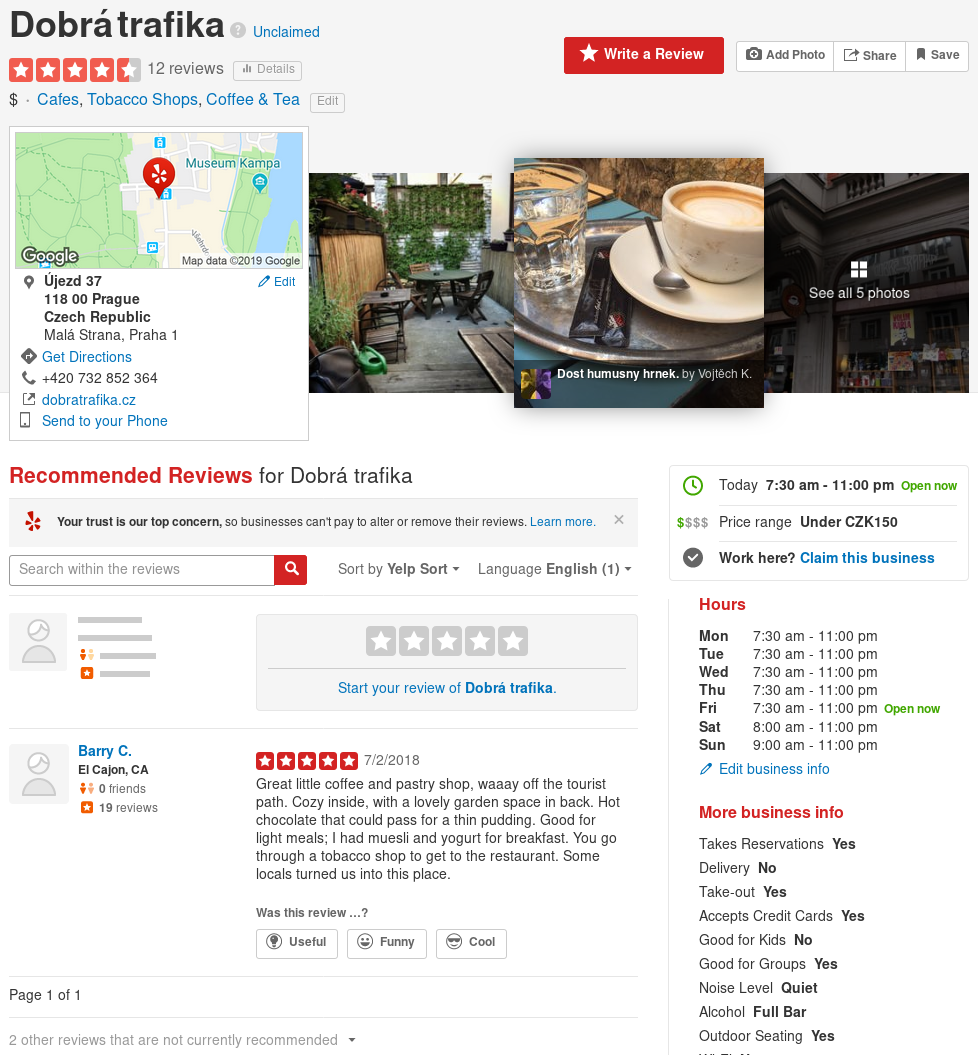
\includegraphics[width=130mm]{../img/dobra_trafika.png}
\caption{An example of an online profile}
\label{fig:dobra_trafika}
\end{figure}

A typical review of a restaurant looks like this:

\begin{code}
Charming decore. Delicious food. Friendly staff.
We'll certainly become repeat customers.
\end{code}

It contains unformatted pieces of information, fragments of sentences or typos.
In general, it can contain anything and \citet{Song14} define it as a new genre --- \textbf{short text}.
Short text is used in e-commerce systems and online communication in general.
It is usually up to 200 characters per document.
It is characterizes by its sparsity, free form and being large-scale and in the real time.
Although an average review in our data has 526 characters, we consider this short text.
First, it fulfills other characteristics.
Second, the bounds are not clearly defined.
An example of another short text system is Instant Messaging software Windows Live Messenger allowing up to 400 characters.

The reasons listed above make it difficult to work with short text.
Furthermore, there are many factors contributing to the difficulty of finding useful reviews.
First, we do not know the author and possibly have only a few reviews by the author.
Also, reviews by the same author can have different quality which is influenced by many factors,
such as the time spent on writing the review or whether the actual experience contains some useful information.
Therefore it is very hard to estimate author's reliability.
Second, reviews are very short, often containing only one piece of information.
Third, a review can quickly become obsolete or irrelevant.
Fourth, what is relevant to some, may not be to others.
All this also makes the task hard even for human operators and as such hard to evaluate our programme selecting useful reviews.

The main reason we chose Yelp is that users can flag properties of other reviews in the form of \emph{likes}.
Each review has three buttons --- \emph{useful}, \emph{funny} and \emph{cool} as can be seen in \Cref{fig:dobra_trafika}.
A user can vote for the property of a review by clicking on one of these buttons.
A typical review flagged as useful looks like this:

\begin{code}
A proper greasy spoon.
I was looking for a bacon flavoured hangover cure and I got one.
And a proper builders mug of tea.
Cheap as chips as well.
\end{code}

It clearly mentions the kind of the restaurant, what to seek there,
who it can be for and price.

On the other hand, a typical not-useful review looks like this:

\begin{code}
Awesome keg.. Always good, even with my own money!
\end{code}

It does only mention the place is good, but does not explain why --- price, friendly staff, location\dots.
The mention about money is unclear.
Does it mean the author has not got much money and therefore appreciate their cheap prices? Or something else?

Sometimes the review is not of a big quality itself, but contains some piece of information which makes it useful.
The review bellow is of a poor quality, not well formatted and only mentioning that we should not go there.
However, the mention about the bouncer and the tip turns out to be very useful for many users,
because it informs about the additional expenses added to the cost.

\begin{code}
Dont bother...this place is a dive!
The bouncer demanded a tip, just to seat us...def seek elsewhere...
you've been warned!!!
\end{code}

Of course, it is often near to impossible to decide whether a review is useful or not.
The review bellow clearly expresses pros and cons.
It is not a place to go when in hurry, not great for some delicious food,
but it is alright when we are not in hurry and want to have a friendly service.
However, the points are somewhat vague and the review is very subjective.

\begin{code}
It was OK. Service was friendly, but slow.
Food was OK, but I don't think it was a good value.
\end{code}


More about the data and the platform can be found in \Cref{app:dataset}.

Our objective is to create a software package that predicts whether some users would flag a restaurant review as a useful.
This prediction can be used for filtering out only useful reviews in a real review system.
We utilize means of supervised binary classification.
The useful likes are used for labelling reviews as \textit{useful} and \textit{not-useful}.
To ensure they have been viewed by enough users to get enough likes,
we take reviews only from a particular time frame
and we use only frequent restaurants with detailed profiles for the same reason.
We focus on classification of English reviews.

This is a well studied field and to date, many approaches to solve this have been introduced.
However, there is no clearly best performing algorithm for particular application.
Our main goal is therefore to compare already existing approaches.
The results can serve as a guide when implementing a real review system.

\section{Roadmap}

In \textbf{\Cref{chap:cls} Text Classification}, we define our task properly as text classification and briefly mention classification in different contexts.
We describe the utilized machine learning methods with examples of concrete usage.

In \textbf{\Cref{chap:fea} Feature Engineering}, we discuss several possibilities how to extract properties called features from text and how to filter only those useful.
Next, we mention dimension reduction as a possibility to reduce the complexity of our solution.
Finally, we introduce several commonly used features and filtering methods.
To a lessen degree, we also talk about non-textual data as well.

In \textbf{\Cref{chap:eval} Evaluation}, we introduce methods for comparing different algorithms.
We describe what requirements we expect a good algorithm to satisfy and how to use the data for comparing performance.
Lastly, we mention commonly used metrics to give us some easily comparable numbers.

In \textbf{\Cref{chap:arch} The Software Project Architecture}, we describe at the conceptual level our software package.
We describe individual modules, how they interact and the overall project structure.
We also talk about different files and configuration the project needs and commands used for running the project.

In \textbf{\Cref{chap:exp} Conducted Experiments}, we outline the experiments.
We describe combinations of algorithms we used and discuss the results.
We justify the compromises made for performance reasons.
Finally, we talk about the impact of size of the data to the performance.

In \textbf{\Cref{app:dataset} Yelp Dataset},
we describe the source of the data and its exact format.
We demonstrate how reviewing of businesses work and
the exact format of the data.

In \textbf{\Cref{app:prepr} Data Preprocessing},
we describe the challenge of obtaining reliable data and
what preprocessing has been done to allow easier manipulation and increase in reliability of the usefulness metrics.

In \textbf{\Cref{app:geneea} Geneea Data},
we describe the NLP analysis used for extracting sentiment and entities.

In \textbf{\Cref{app:techn} Package Technicalities},
we describe technical details and peculiarities of the software package.
We also provide commands for running the experiments and specify configuration.

In \textbf{\Cref{app:mi} Top Features by Mutual Information},
we list mutual information of selected features.


\section{Typographic Conventions}

In this thesis, we use the following typographic conventions:

\begin{itemize}
\item \textbf{bold} for definitions of new terms

\item \textit{italics} for mentions of already defined names. It also denotes data files in \Cref{chap:arch}.

\item \texttt{monospace} is used for code and filenames. It is used for process names in \Cref{chap:arch}.

\end{itemize}

\section{Related Work}

A lot of research has been done in short text classification.
Executive summary can be found in \citet{Song14}.
They define short text as a new genre; listing its characteristics, summarizing possible approaches to short text classification and evaluating performance.

One of the well studied dataset is tweets from Twitter.\footnote{\url{https://twitter.com}}
A lot of studies on sentiment analysis have been conducted.
\citet{jiang2011target} allege that most approaches follow
\citet{pang2002thumbs} who utilize machine learning based classifiers;
the state-of-the-art being \citet{go2009twitter} and \citet{barbosa2010robust}.
Perhaps more relevant study on Twitter is \citep{sriram2010short},
which tackles the problem of filtering relevant information.

Reviews are to author's knowledge less studied.
One of the relevant papers is \citet{ganu2009beyond}.
They discuss the difficulties of selecting useful restaurant reviews.
Unlike this thesis, they do not classify reviews as a whole, but instead try to find reviews containing topics such as food or service.
The main attempt is to find some structure in the free form.

Related text classification research focuses on sentiment analysis and toxic speech detection.
A lot of research is focusing on sentiment analysis.

Relatively close research focuses on toxic speech.
\citet{van2018challenges} talk about toxic speech as non-constructive and non-inclusive conversation including hate speech, threats, insults and in general fruitless conversation.
Filtering out fruitless text is our focus to high extent too.
Apart from already mentioned challenges they mention high variance in performance and difficulty to define the topic clearly.
Basic review of toxic speech classification can be found in \citet{gunasekara2018review}.
